% ********** BEGIN Chapter 3 **********
\chapter{Study}
\label{sec:BackgroundStudy}


\section{VoIP Market}
\label{sec:BackgroundStudy:VoIPMarket}

In the telecom market, VoIP technology has gained more and more customers. The advantage of VoIP is obviously, much cheaper fee and almost same quality as traditional telephone.  Report from \textsf{Infonetics} indicates that, in the year 2007, the subscribers for VoIP are under 80 all around world. Most of them are in the Asia Pacific region. However by the year of 2011 the user will be 135 million, predicted by \textsf{MarketResearch.com}. And a UK research company \textsf{Disruptive Analysis Ltd.} predicts the users of mobile-VoIP will be 250 million by the year of 2012.\cite{StateOfTheVoIPMarket2008}

The analyses and figures above draw a brilliant future of VoIP market.  

\subsection{VoIP Service Provider}
\label{sec:BackgroundStudy:VoIPMarket:VoIPServiceProvider}

VoIP service provider is the company which supplies the products of VoIP/PSTN gateway. Or the ones who supply the service that customers can call a PSTN phone by a VoIP phone via their service/network. There are hundreds of such companies in the world. 


\subsection{VoIP Client}
\label{sec:BackgroundStudy:VoIPMarket:VoIPClient}

A VoIP client is a common SIP client software or a IMS client software. This kind of software runs on a computer or mobile device and implements the SIP or/and IMS standard. It can work like a phone to dial or answer VoIP calls.  

\subsection{Solution Provider}
\label{sec:BackgroundStudy:VoIPMarket:SolutionProvider}

A solution provider is a company that supplies both VoIP service and software client, such as \textsf{Skype}\texttrademark{}\footnote{\url{http://www.skype.com}}, \textsf{VoipStunt}\footnote{\url{http://www.voipstunt.com}} and JAJAH\footnote{\url{http://www.jajah.com}}.  Among them \textsf{Skype} is the most famous one. It has a very good quality of voice and functionality client. However, the \textsf{Skype} is not following the standard of SIP. So it means, only the \textsf{Skype} client itself can use the service of \textsf{Skype}. \textsf{VoipStund} and \textsf{JAJAH} supply relevant lower fee and less quality of audio.


\section{Third Party Call Control}
\label{sec:BackgroundStudy:ThirdPartyCallControl}

In the traditional telephony context, third party call control allows one entity (which we call the controller) to set up and manage a communications relationship between two or ore other parties.  Third party call control (referred to as \textbf{3pcc}\label{sym:3pcc}) is often used for operator services (where an operator creates a call that connects two participants together) and conferencing.\cite{RFC3725}

\begin{figure}[!hbtp]
\centering
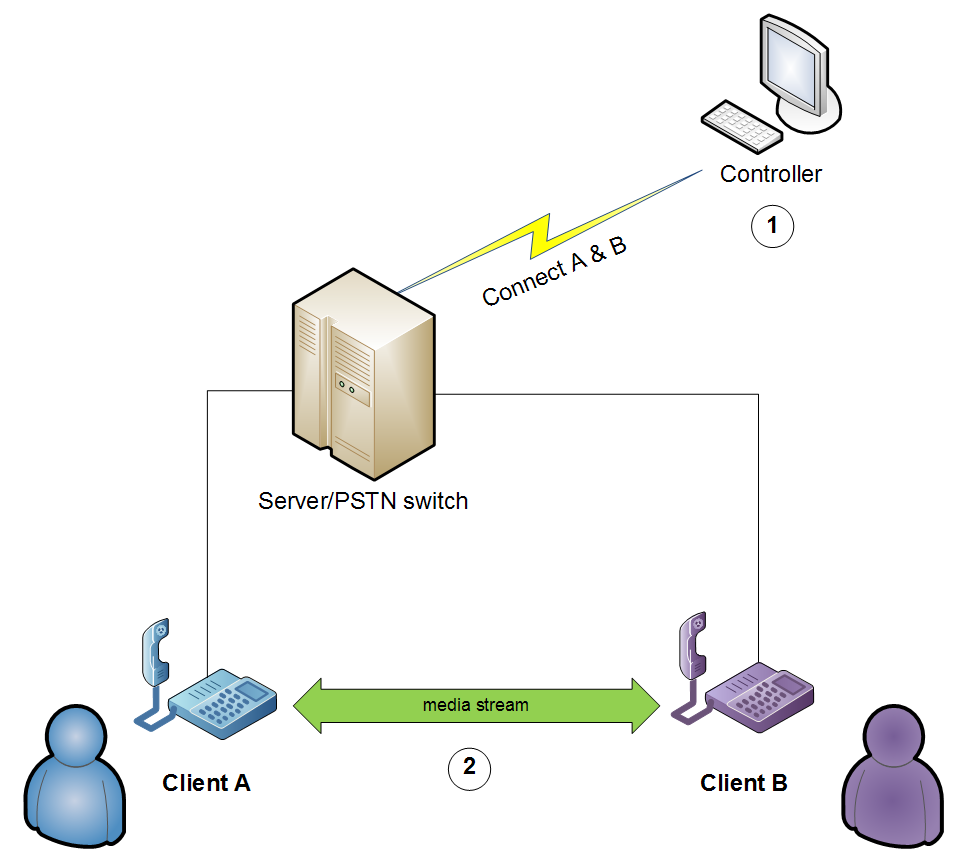
\epsfig{file=chap03/resources/3pcc, width=4in}
\caption{Third party call control}
\label{fig:ThirdPartyCallControl}
\end{figure}

A general work flow of 3pcc is shown in Figure \ref{fig:ThirdPartyCallControl}. The initial side of the phone is the \textit{controller}. The \textit{controller} sends a signal ``connect \textit{client \nolinebreak A} and \textit{client \nolinebreak B}'' to the server \hyperref[fig:ThirdPartyCallControl]{\ding{172}}. And the server establishes a call between \textit{client A} and \textit{B} \hyperref[fig:ThirdPartyCallControl]{\ding{173}}.


\section{Why Web Call Example Application?}
\label{sec:BackgroundStudy:WhyWebCallExampleApplication}

Based on IMS/SIP technology, Web Call Example Application integrated call functions into Web containers. This presents a simple way to implement the communication convergence of Web, IMS/SIP network, and CS networks. It does not require the installation of the plug-in clients on the browser or other special client software as most VoIP services.

The Web Call Example Application is nether a service provider or a client that described above. It is more like a controller which acts as a initial side in third party call control. That is, it support all standard client and service provider. Another advantage of Web Call Example Application is that The desktop view, mobile browser view and JavaME client all share a same database. The user can access a same contact book and use a same service account from different platform. None of the solution provider or client have the same function.







% ********** End of chapter 3 **********
